\documentclass[10pt,a4paper,english]{article}
\usepackage{abstract}
\usepackage{multicol}

% Phonetics
\usepackage{tipa}

\usepackage[left=2.7cm,right=2.7cm,top=2cm,bottom=2cm]{geometry}
\usepackage[utf8]{inputenc}
\usepackage[USenglish]{babel}
\usepackage[T1]{fontenc}
\usepackage{csquotes}
\usepackage{float}
\usepackage[bottom]{footmisc} % keep footnotes at the bottom of the page
\usepackage{setspace} % to have the \setstretch{baselinestrech} command available
\usepackage{ragged2e} % text alignment
\usepackage[parfill]{parskip} % no indentation for paragraphs, instead add spacing
\usepackage{pdfpages} %for including pdf

% Easy tables, e.g. for coloring columns as seen here.
% https://tex.stackexchange.com/a/613906/
% \usepackage{tabularray}
\usepackage{subfigure}
\usepackage{booktabs}

% Graphics & Color
\usepackage{xcolor}
\definecolor{heidelberg-red}{HTML}{E50A37}
\usepackage{graphicx}
\usepackage{caption}

% Math & Physics
\usepackage{amsmath}
\usepackage{amsfonts}
\usepackage{amsthm}
\usepackage{amssymb}
\usepackage{bm}
\usepackage{cancel}

\usepackage{witharrows} % http://mirrors.ibiblio.org/CTAN/macros/generic/witharrows/witharrows.pdf
\usepackage{nicefrac} % usage: \nicefrac{nominator}{denominator}
\usepackage{physics}
\usepackage{siunitx}
\sisetup{
	locale=US,
	group-separator={,},
	group-digits=integer,
	quotient-mode=fraction,per-mode=symbol}
\usepackage{empheq} % boxed equations: https://trucastuces.wordpress.com/2012/10/10/boxed-equations-in-latex/

% Acronyms
\usepackage[automake]{glossaries}
\setacronymstyle{long-short}

\usepackage{lmodern}
\usepackage{fancyhdr}
\usepackage{enumerate}
% we use the option hidelinks here to avoid ugly borders around clickable items, e.g. links and cross-references
\usepackage{hyperref} % clickable links
\hypersetup{
	colorlinks = true,
	linkcolor={red!50!black}, % Color of internal links
	citecolor={blue!50!black}, % Color of citations
	urlcolor={blue!80!black} % Color for external hyperlinks
}
\usepackage{todonotes}
\setlength {\marginparwidth }{2cm}      % margin for todo notes
\usepackage[nameinlink]{cleveref}

\let\qty\SI % see "bug" (warning) in https://tex.stackexchange.com/a/628184

% Enumerations
\usepackage{enumitem}
% Enumerate lists as a) b) instead of 1. 2.
\setenumerate[0]{label=\textbf{\alph*)}}
% remove indentation of enumerate environment
\setlist{leftmargin=*}

% ---- Algorithms ----
\usepackage{float}
% http://tug.ctan.org/macros/latex/contrib/algorithm2e/doc/algorithm2e.pdf
\usepackage[ruled, algosection, lined, scleft, linesnumbered, noend]{algorithm2e}
\renewcommand{\algorithmautorefname}{Algorithm}

% Algorithm comments
\newcommand\mycommentsfont[1]{\footnotesize\ttfamily{#1}}
\SetCommentSty{mycommentsfont} % https://tex.stackexchange.com/a/162208/
\SetKwComment{Comment}{$\triangleright$\ }{} % https://tex.stackexchange.com/a/200736/
\SetKwRepeat{DoWhile}{do}{while}

% Function/Procedure
\SetKwProg{Fn}{Function}{:}{}
\SetArgSty{textnormal}

% Keywords
\SetKw{Continue}{continue} % https://tex.stackexchange.com/a/298503/
\SetKw{Break}{break}

% Code
% https://stackoverflow.com/a/79057262/
\usepackage[most]{tcolorbox}
\tcbset{
    frame empty,
    colback=lightgray!20
}

% Bibliography
\usepackage[
    backend=biber,
    style=numeric,
    sorting=none
]{biblatex}

\addbibresource{literature.bib}
\addbibresource{data.bib}

% for convenience
% usage: \q{I am citing} in order to get "I am citing"
\newcommand{\q}[1]{\enquote{#1}}

\newcommand{\set}[1]{\ensuremath{\{\,#1\,\}}}
\newcommand*{\coloniff}{\ratio\Leftrightarrow}
\newcommand*{\colonLeftrightarrow}{\ratio\Leftrightarrow}
\renewcommand{\implies}{\Rightarrow}
\renewcommand{\impliedby}{\Leftarrow}
\renewcommand{\iff}{\Leftrightarrow}
\newcommand{\definedAs}{\ratio\Leftrightarrow}
\newcommand{\perc}[1]{\ensuremath{\qty{#1}{\percent}}}
\newcommand{\solution}[1]{\ensuremath{\underline{\underline{#1}}}}
\newcommand{\determ}{\operatorname{det}}
\newcommand{\R}{\mathbb{R}}

\DeclareMathOperator*{\argmin}{arg\,min}

% German specific
\newcommand{\zB}{z.\,B. }
\newcommand{\eg}{e.\,g. }
\newcommand{\dash}{d.\,h. }
\newcommand{\ie}{i.\,e. }

% Text over equal sign, e.g. to indicate that a specific definition was used
% usage: \eqdef{text over equal sign}
% https://tex.stackexchange.com/a/74132
\newcommand{\eqdef}[1]{\mathrel{\overset{\makebox[0pt]{\mbox{\normalfont\tiny\sffamily #1}}}{=}}}
\newcommand{\impliesdef}[1]{\mathrel{\overset{\makebox[0pt]{\mbox{\normalfont\tiny\sffamily #1}}}{\implies}}}
% https://tex.stackexchange.com/questions/9466/color-underline-a-formula
\newcommand{\mline}[2][red]{\color{#1}\underline{{\color{black}#2}}\color{black}}

% Math environments
\newenvironment{eqarrows}{
	\begin{equation}
		\begin{WithArrows}
		}{%
		\end{WithArrows}
	\end{equation}
	\ignorespacesafterend
}
\newenvironment{eqarrows*}[1][]{
	\begin{equation*}
		\begin{WithArrows}[#1]
		}{%
		\end{WithArrows}
	\end{equation*}
	\ignorespacesafterend
}
\newenvironment{eqboxed*}{
	% https://tex.stackexchange.com/questions/419132/newenvironment-with-empheq-inside-tcolorbox
	\empheq[box=\fbox]{align*}
	}{%
	\endempheq%
	\ignorespacesafterend
}

% Coding
\newcommand\Cpp{C\nolinebreak[4]\hspace{-.05em}\raisebox{.4ex}{\relsize{-3}{\textbf{++}}}}

% Other math stuff
% vector with prime symbol
\newcommand{\vecp}[1]{\ensuremath{\vec{#1}^{\,\prime}}}
\newcommand{\dvecp}[1]{\ensuremath{\dvec{#1}^{\,\prime}}}
\newcommand{\ddvecp}[1]{\ensuremath{\ddvec{#1}^{\,\prime}}}
% vector prime with subscript
\newcommand{\vecps}[2]{\ensuremath{\vec{#1}^{\,\prime}_{\!#2}}}

% copied from https://tex.stackexchange.com/a/44071/249769
% Macro \xvec
\makeatletter
\newlength\xvec@height%
\newlength\xvec@depth%
\newlength\xvec@width%
\newcommand{\xvec}[2][]{%
	\ifmmode%
	\settoheight{\xvec@height}{$#2$}%
	\settodepth{\xvec@depth}{$#2$}%
	\settowidth{\xvec@width}{$#2$}%
	\else%
	\settoheight{\xvec@height}{#2}%
	\settodepth{\xvec@depth}{#2}%
	\settowidth{\xvec@width}{#2}%
	\fi%
	\def\xvec@arg{#1}%
	\def\xvec@dd{:}%
	\def\xvec@d{.}%
	\raisebox{.2ex}{\raisebox{\xvec@height}{\rlap{%
				\kern.05em%  (Because left edge of drawing is at .05em)
				\begin{tikzpicture}[scale=1]
					\pgfsetroundcap
					\draw (.05em,0)--(\xvec@width-.05em,0);
					\draw (\xvec@width-.05em,0)--(\xvec@width-.15em, .075em);
					\draw (\xvec@width-.05em,0)--(\xvec@width-.15em,-.075em);
					\ifx\xvec@arg\xvec@d%
					\fill(\xvec@width*.45,.5ex) circle (.5pt);%
					\else\ifx\xvec@arg\xvec@dd%
					\fill(\xvec@width*.30,.5ex) circle (.5pt);%
					\fill(\xvec@width*.65,.5ex) circle (.5pt);%
					\fi\fi%
				\end{tikzpicture}%
	}}}%
	#2%
}
\makeatother

% --- Override \vec with an invocation of \xvec.
\let\stdvec\vec
\let\ovec\vec
\renewcommand{\vec}[1]{\xvec[]{#1}}
% --- Define \dvec and \ddvec for dotted and double-dotted vectors.
\newcommand{\dvec}[1]{\xvec[.]{#1}}
\newcommand{\ddvec}[1]{\xvec[:]{#1}}


\renewcommand{\abstractnamefont}{\normalfont\bfseries}
\renewcommand{\abstracttextfont}{\normalfont\small\itshape}

\title{\vspace{-1em}Similarity between French words based on their phonetic transcription using Needleman-Wunsch \& graph clustering}
\author{Dominic Plein}
\date{February 17, 2025}

\newcommand{\abstractText}{\noindent
	\newline\noindent
	This project is part of the \href{https://membres-ljk.imag.fr/Christophe.Picard/teaching/gp-gpu}{GP-GPU Computing course} at UGA by Christophe Picard.
    Lorem ipsum dolor sit amet, consetetur sadipscing elitr.
    Lorem ipsum dolor sit amet, consetetur sadipscing elitr, sed diam nonumy eirmod tempor invidunt ut labore et dolore magna aliquyam erat, sed diam voluptua. At vero eos et accusam et justo duo dolores et ea rebum. Stet clita kasd gubergren, no sea takimata sanctus est Lorem ipsum dolor sit amet. Lorem ipsum dolor sit amet, consetetur sadipscing elitr, sed diam nonumy eirmod tempor invidunt ut labore et dolore magna aliquyam erat, sed diam voluptua. At vero eos et accusam et justo duo dolores et ea rebum. Stet clita kasd gubergren, no sea takimata sanctus est Lorem ipsum dolor sit amet. Lorem ipsum dolor sit amet, consetetur sadipscing elitr, sed diam nonumy eirmod tempor invidunt ut labore et dolore magna aliquyam erat, sed diam voluptua. At vero eos et accusam et justo duo dolores et ea rebum. Stet clita kasd gubergren, no sea takimata sanctus est Lorem ipsum dolor sit amet.
}

% Acronyms
\makeglossaries
\newacronym{ipa}{IPA}{International Phonetic Alphabet}
\newacronym{pos}{POS}{Part-of-Speech}
\newacronym{ptx}{PTX}{Parallel Thread Execution}

\begin{document}

\setlength{\abovedisplayskip}{0.2em}
%\setlength{\belowdisplayskip}{0pt}
%\setlength{\abovedisplayshortskip}{0pt}
%\setlength{\belowdisplayshortskip}{0pt}

% Title & Abstract
\maketitle
\begin{abstract}
    \abstractText
    \newline
    \newline
\end{abstract}
% \twocolumn[
%   \begin{@twocolumnfalse}
%     \maketitle
%     \begin{abstract}
%       \abstractText
%       \newline
%       \newline
%     \end{abstract}
%   \end{@twocolumnfalse}
% ]

% Content
% \setcounter{section}{1}

% \pagebreak

\begin{multicols*}{2}
\tableofcontents
\section{Introduction}

The \gls{ipa} uses special symbols\footnote{See for example the French list \href{https://en.wikipedia.org/wiki/Help:IPA/French}{here}.} to represent the sound of a spoken language \cite{ipa}. This is useful for language learners since the pronunciation of a word can be significantly different from its written form. For example, the French word \textit{renseignement} (information) is pronounced \textipa{/K\~{a}.sE\textltailn.m\~{a}/}. Based on this alphabet, one might wonder if we can construct a metric that quantifies the \textbf{similarity between two words based on their phonetic transcription}. This would allow to construct a graph where nodes are words and undirected edges are weighted by the distance between the words. Such a graph can be used to find neighbors of a word based on the respective phonetic similarity. This opens up the possibility to apply clustering algorithms and other methods stemming from graph theory in order to analyze the phonetic structure of a language.

Calculating the distance between each pair of words corresponds to a fully-connected graph. Our dataset consists of around 600,000 French words and their \gls{ipa} transcription, alongside their frequency in the French language. Excluding self-loops, we find a vast number of edges \eqref{eq:num-edges}:
\begin{align}
    \text{\#nodes} &= 600,000 \\
    \text{\#edges} &= \frac{600,000 \cdot 599,999}{2} \approx \num{1.8e11}
\end{align}
This high number and the independent nature of the distance calculation for each pair of words makes the problem well-suited for parallelization. In \autoref{sec:needleman-wunsch}, we present the Needleman–Wunsch algorithm used to calculate the distance between two words. In \autoref{sec:impl}, we discuss how to parallelize this algorithm on a CPU using the \textit{Rayon} library in Rust and on a consumer Nvidia GPU using the CUDA framework with the \textit{cudarc} Rust library. Finally, we present performance results and provide visualizations of the obtained graphs in \autoref{sec:eval}. We conclude in \autoref{sec:conclusion} and discuss how this method can be improved and how future work could extend it.

% In the following, by \textit{word} we always refer to its phonetic transcription. That is, homophones like the French words \textit{vert} \textipa{/vEK/} (green) and \textit{verre} \textipa{/vEK/} (glass) are considered the same word.

% \vfill\null

\newcolumn
\section{Needleman-Wunsch}
\label{sec:needleman-wunsch}
\newcommand{\lenn}{\text{len}}

The Needleman-Wunsch algorithm (developed by Saul B. Needleman and Christian D. Wunsch in 1970) calculates the global alignment of two strings and was originally used in bio-informatics to compare DNA sequences. For our purposes, the alphabet will instead consist of the phonetic \gls{ipa} symbols. Out of all possible alignments of two words (including gaps), the Needleman-Wunsch algorithm finds the one with the smallest distance, \ie the alignment with the highest \q{score}. The algorithm is based on dynamic programming and has a time complexity of $\mathcal{O}(\lenn(A) \cdot \lenn(B))$, where $A$ and $B$ are the two words to be compared.

\autoref{alg:needleman-wunsch} features the pseudo-code of the score computation\footnote{The respective \href{https://en.wikipedia.org/wiki/Needleman\%E2\%80\%93Wunsch_algorithm}{Wikipedia page} also provides a good introduction. Furthermore, the score matrix is interactively explained in the \href{https://bioboot.github.io/bimm143_W20/class-material/nw/}{Global Alignment App}.}. In \autoref{fig:matrix-nuance-puissance-optimal}, we see the resulting score matrix that the algorithm constructed for the French words \textit{puissance} and \textit{nuance}. Follow the indicated path (red tiles) from the bottom right to the top left to find the (reversed) optimal alignment (see \autoref{tab:nuance-puissance-alignment-optimal});

\begin{table}[H]
\centering
\begin{tabular}{l*{6}{>{\centering\arraybackslash}p{0.2cm}}}
    \toprule
    \textit{puissance}
    & \textipa{p} & \textipa{\textturnh} & \textipa{i} & \textipa{s} & \textipa{\~A} & \textipa{s}\\
    \midrule
    \textit{nuance}
    & \textipa{n} & \textipa{\textturnh} & -- & -- & \textipa{\~A} & \textipa{s}\\
    \bottomrule
\end{tabular}
\caption{The optimal alignment yields a score of $-2$. See the path in \autoref{fig:matrix-nuance-puissance-optimal}.}
\label{tab:nuance-puissance-alignment-optimal}
\end{table}

\begin{figure}[H]
    \centering
    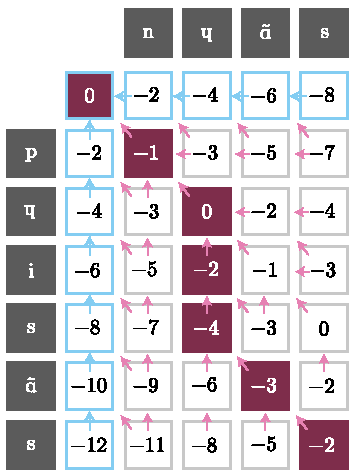
\includegraphics[width=0.77\linewidth]{assets/illustrator/matrix-nuance-puissance-optimal.pdf}
    \caption{Needleman-Wunsch score matrix for the words $A\coloneqq\textit{puissance}$ \textipa{/p\textturnh is\~As/} (power, strength) and $B\coloneqq\textit{nuance}$ \textipa{/n\textturnh\~As/} (nuance, shade). The arrows indicate which steps locally maximize the score. The red tiles trace the path of the optimal alignment. Match Score: $1$, Mismatch Score: $-1$, Gap Penalty: $p=-2$.}
    \label{fig:matrix-nuance-puissance-optimal}
\end{figure}

\vfill\null

We first discuss the meaning of the different steps (arrows) in the score matrix (\autoref{fig:matrix-nuance-puissance-optimal}) to then explain how to construct this matrix.

\begin{itemize}

    \item In a \textbf{diagonal step}, both symbols that indicate the current position in the two words change. Such a step corresponds to either a match or a mismatch between the two symbols. In the example, the \textipa{/s/} symbols in the bottom-right corner match, which is why the step beforehand is a \textit{diagonal} step from the field $-3$ to $-2$. The score increases by $1$ since we defined the match score to be $+1$ (and a mismatch score as $-1$).

    \item In a \textbf{vertical} or \textbf{horizontal step}, only one of the two symbols changes. We interpret this as a gap in the alignment, \ie one symbol aligns to a gap in the other word. In the example, this is the case two times when we move from the red field $0$ down to $-2$ and then down to $-4$. The score decreases by $2$ each time, as we defined the gap penalty as $p \coloneqq -2$ in this example. The gap is indicated by \q{--} in the alignment (see \autoref{tab:nuance-puissance-alignment-optimal}). As we are still in the column of \textipa{/\textturnh/} of the word \textipa{/n\textturnh\~As/}, we insert two \q{--} symbols after the \textipa{/\textturnh/} in \autoref{tab:nuance-puissance-alignment-optimal}. This step is sometimes also referred to as \textbf{deletion} or \textbf{insertion}.
    
\end{itemize}

To find the score matrix for given input words $A$ and $B$, we follow \autoref{alg:needleman-wunsch}. First, the score matrix of dimension $(\lenn(A)+1) \times (\lenn(B)+1)$ is initialized\footnote{This does not necessarily involve setting all fields to $0$ as will become clear.}. Then, in lines~\ref{algstep:init-gap-start} to~\ref{algstep:init-gap-end}, the blue-bordered tiles of \autoref{fig:matrix-nuance-puissance-optimal} are filled with the gap penalty $p$ times the index. This is necessary since the only possible step for these tiles is either a vertical or horizontal step (blue arrows), thus leading to a gap in the alignment as discussed beforehand that we punish with the gap penalty $p$.

\begin{figure}[H]
    \centering
    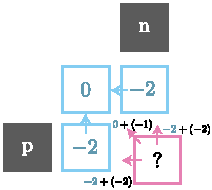
\includegraphics[width=0.5\linewidth]{assets/illustrator/matrix-nuance-puissance-subcalc.pdf}
    \caption{Calculations for one element of the Needleman-Wunsch score matrix.}
    \label{fig:matrix-nuance-puissance-subcalc}
\end{figure}

In the nested loops (lines~\ref{algstep:nested1} and~\ref{algstep:nested2}), we then iterate over the remaining fields of the score matrix (index now starts at $1$, not $0$) which corresponds to traversing the matrix row-wise. To each field, we assign the maximum of three values:

% \vfill\null
% \columnbreak

\begin{algorithm*}
    \DontPrintSemicolon
    
    \SetKwFunction{calcScoreFunc}{calculateScore}
    \SetKwData{WordA}{$A$}
    \SetKwData{WordB}{$B$}
    \SetKwData{Sim}{similarity}
    \SetKwData{GapPenalty}{$p$}
    \SetKwData{ScoreMatrix}{scoreMatrix}
    \newcommand{\ScoreMatrixIdx}[2]{{\ScoreMatrix}[{#1}][{#2}]}
    \SetKwData{Cost}{cost}
    \SetKwData{MatchScore}{matchScore}
    \SetKwData{DeleteScore}{deleteScore}
    \SetKwData{InsertScore}{insertScore}
    \SetKwData{Score}{score}
    \SetKwFunction{len}{len}

    \KwIn{
        $\WordA = \set{A_0, \ldots, A_{\len(A)-1}}$,
        $\WordB = \set{B_0, \ldots, B_{\len(B)-1}}$,\\
        \qquad\qquad \Sim: similarityScoreFunc,
        \GapPenalty: GapPenalty
    }
    \KwOut{\Score}
    \Fn{\calcScoreFunc{}}
    {
        Init \ScoreMatrix with dimensions $(\len(\WordA)+1) \times (\len(\WordB)+1)$\;

        \BlankLine

        \For{$i \in \{0, \ldots, \len(\WordA)\}$\label{algstep:init-gap-start}}
        {
            \ScoreMatrixIdx{$i$}{$0$} $\gets \GapPenalty \cdot i$\;
        }
        \For{$j \in \{0, \ldots, \len(\WordB)\}$}
        {
            \ScoreMatrixIdx{$0$}{$j$} $\gets \GapPenalty \cdot j$
            \label{algstep:init-gap-end}\;
        }

        \BlankLine

        \For{$i \in \{1, \ldots, \len(\WordA)\}$\label{algstep:nested1}}
        {
            \For{$j \in \{1, \ldots, \len(\WordB)\}$\label{algstep:nested2}}
            {
                \Cost $\gets$ $\Sim(\WordA_{i-1}, \WordB_{j-1})$\;
                \MatchScore $\gets$ \ScoreMatrixIdx{$i-1$}{$j-1$} + \Cost
                \label{algstep:matchscore}\;
                \DeleteScore $\gets$ \ScoreMatrixIdx{$i-1$}{$j$} + \GapPenalty
                \label{algstep:deletescore}\;
                \InsertScore $\gets$ \ScoreMatrixIdx{$i$}{$j-1$} + \GapPenalty
                \label{algstep:insertscore}\;
                \ScoreMatrixIdx{$i$}{$j$} $\gets$ $\max(\MatchScore, \DeleteScore, \InsertScore)$\;
            }
        }

        \BlankLine

        \Return\! \ScoreMatrixIdx{$\len(\WordA)$}{$\len(\WordB)$}\;
    }
    
    \caption{Needleman-Wunsch}
    \label{alg:needleman-wunsch}
\end{algorithm*}

\begin{itemize}

    \item The \textbf{match score} is calculated by checking the step to the upper left diagonal (\autoref{algstep:matchscore}). In the example of \autoref{fig:matrix-nuance-puissance-subcalc}, this would result in a value $0+(-1) = -1$, where $0$ is the value in the upper left diagonal field and $-1$ is the cost of the mismatch between \textipa{/p/} and \textipa{/n/}. In case of a match, the new value would be $0 + 1 = 1$. In the algorithm, we also consider the case where costs for a match and a mismatch depend on the symbols themselves, which is why we introduce the function \tcboxverb{similarity} that returns the cost of aligning two symbols. This is especially useful when comparing phonetic symbols, as the similarity between two symbols can be defined in a more sophisticated way than just $1$ or $-1$ (\eg replacing a vowel with a consonant might be more costly than replacing a vowel with another vowel).
    
    \item The \textbf{delete score} refers to the step from the field above (\autoref{algstep:deletescore}). In the example, we find $(-2) + (-2) = -4$ as new value ($-2$ is the value in the field above and $p=-2$ is the gap penalty). This steps signifies that a symbol in word A aligns to a gap in word B (here: \textipa{/i/} and \textipa{/s/} of \textit{puissance} align to gaps in \textit{nuance}).
    
    \item The \textbf{insert score} refers to the step from the left (\autoref{algstep:insertscore}). In the example, we find $(-2) + (-2) = -4$ as new value ($-2$ is the value in the field to the left and $p=-2$ is the gap penalty). This steps signifies that a symbol in word B aligns to a gap in word A (this does not occur in the example).

\end{itemize}

The new value of the current field is then the maximum of the three values, such that we locally maximize the score: $\max(-1, -4, -4) = -1$. In \autoref{fig:matrix-nuance-puissance-optimal}, we additionally kept track of the steps that led to the optimal alignment by means of the rose arrows (here only the diagonal step that yields the new maximal score of $-1$). For our purposes, we don't want to reconstruct the exact alignment that led to the optimal score, but only the score itself. Thus, we can omit the backtracking step and don't need to store the rose arrows.

By construction, \textbf{the bottom-right field of the score matrix contains the score of the optimal alignment} (in our case $-2$, see \autoref{tab:nuance-puissance-alignment-optimal}). This is ensured by the Principle of Optimality (Richard Bellman), which states that an optimal solution to a problem can be constructed from optimal solutions to its subproblems. In the context of the Needleman-Wunsch algorithm, this means that the optimal alignment score for two sequences can be derived by considering the optimal alignment scores of progressively smaller subsequences. Each cell in the score matrix represents the optimal alignment score for the corresponding prefixes of the two sequences up to that point, since we take the maximum of the three possible steps (match, delete, insert) at each cell. This ensures that the final cell (in the bottom right) contains the optimal score for the entire sequences.

\autoref{tab:nuance-puissance-alignment-non-optimal} shows an example of a non-optimal alignment of the two words, yielding a score of $-15$ (compared to $-2$ for the optimal path). \autoref{fig:matrix-nuance-puissance-non-optimal} depicts the corresponding score matrix. Note how the indicated path includes 4 non-optimal choices (yellow strokes).

\begin{table}[H]
    \centering
    \begin{tabular}{l*{9}{>{\centering\arraybackslash}p{0.2cm}}}
        \toprule
        \textit{puissance}
        & -- & \textipa{p} & \textipa{\textturnh} & -- & \textipa{i}
        & -- & \textipa{s} & \textipa{\~A} & \textipa{s}\\
        \midrule
        \textit{nuance}
        & \textipa{n} & -- & \textipa{\textturnh} & \textipa{\~A} & --
        & \textipa{s} & -- & -- & --\\
        \bottomrule
    \end{tabular}
    \caption{This non-optimal alignment yields a score of $-15$. See the path in \autoref{fig:matrix-nuance-puissance-non-optimal}.}
    \label{tab:nuance-puissance-alignment-non-optimal}
\end{table}
    
\begin{figure}[H]
    \centering
    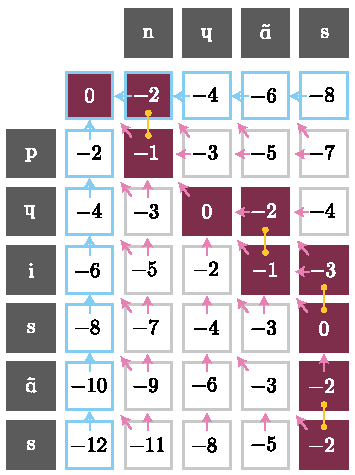
\includegraphics[width=0.77\linewidth]{assets/illustrator/matrix-nuance-puissance-non-optimal.pdf}
    \caption{Needleman-Wunsch score matrix and the path (in red) for a non-optimal alignment. All parameters are the same as in \autoref{fig:matrix-nuance-puissance-optimal}.}
    \label{fig:matrix-nuance-puissance-non-optimal}
\end{figure}

\begin{figure*}
    \centering
    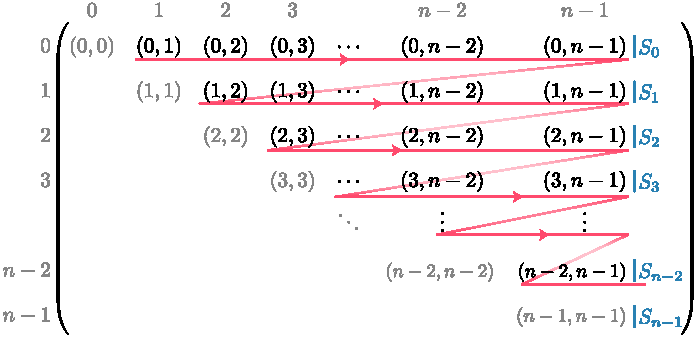
\includegraphics[width=0.78\textwidth]{assets/illustrator/traverse-schema.pdf}
    \caption{Row-major traversal of the adjacency matrix. $n$ is the total number of words (\ie nodes).}
    \label{fig:traverse-schema}
\end{figure*}

\section{Data Preparation}
\label{sec:data}

We use the \href{https://github.com/frodonh/french-words}{\textbf{french-words}} dataset (frodonh, 2020), which contains 691,969 French words. It is compiled from several sources including (among others) the Debian package \href{https://packages.debian.org/fr/sid/wfrench}{wfrench} (used for spell checking), \href{http://www.lexique.org/}{Lexique 3.83} (Boris New \& Christophe Pallier), the \href{https://infolingu.univ-mlv.fr/DonneesLinguistiques/Dictionnaires/telechargement.html}{DELA dictionary} from the University of Marne-la-Vallée as well as the \href{https://github.com/hbenbel/French-Dictionary}{French-Dictionary} (Hussem Ben Belgacem). The words also include \acrfull{pos} tagging information, \eg whether it is a noun, verb, adjective, preposition etc. It also comprises the usage frequency according to Lexique.org and Google Ngrams. We use the average of both sources (or just one if the other is missing).

Since the french-words dataset does not include the phonetic transcriptions, we consult the \href{https://github.com/DanielSWolf/wiki-pronunciation-dict}{\textbf{wiki-pronunciation-dict}} (Daniel Wolf, 2021) extracted from the French \href{https://fr.wiktionary.org/}{Wiktionnaire}. We merge both datasets to obtain 611,786 words with their \gls{ipa} transcription. If multiple phonetic transcription are available, we only store the first one. For easy access, we store the data in a dataclass and serialize it to a pickle file of around \qty{60}{\mega\byte}.

Additionally, we extract all used phonetic symbols and assign integer IDs to them. This enables us to store the transcription as a list of integers. For our examples, we obtain \autoref{tab:phonetic-encoding}. The Needleman-Wunsch algorithm will then work on these integer lists. Note that we consider \textipa{/dZ/} as one symbol, even though it is a combination of \textipa{/d/} and \textipa{/Z/}. The same applies to \textipa{/tS/}. This is to account for the different pronunciation of the combined symbols compared to the individual ones.

% \vspace{-0.2em}

\begin{table}[H]
    \centering
    \begin{tabular}{lll}
    \toprule
    \textbf{Word} & \textbf{\acrshort{ipa}} & \textbf{Encoding} \\
    \midrule
    \textit{puissance} & \textipa{/p\textturnh is\~As/} & $[0,18,16,11,26,11]$ \\
    \textit{nuance} & \textipa{/n\textturnh\~As/} & $[29,18,26,11]$ \\
    \bottomrule
    \end{tabular}
    \caption{Example of two words with their phonetic transcription and encoding.}
    \label{tab:phonetic-encoding}
\end{table}

\section{Parallelized algorithm}
\label{sec:impl}

test

\vfill\null
% \pagebreak
\columnbreak
\section{Evaluation}
\label{sec:eval}

We deploy our GPU code on a consumer Nvidia GeForce GTX 1060\footnote{We use the Driver Version 572.42 and CUDA Toolkit 12.8 inside WSL2 (Ubuntu 22.04 jammy).} with 6GB GDDR5. Every code change related to the GPU code is verified by comparing the resulting binary edge weights file with the one generated by our parallelized Rust implementation on the CPU. This baseline helps to quickly identify errors, which could otherwise remain unnoticed. During our tests, we define a manual threshold to cap the number of words to a user-defined threshold. The words considered are sorted according to their frequency as we are interested in relationships between the most commonly used words.

\textbf{Performance.} A fair comparison between the CPU and GPU implementation is not possible since focus was put in optimizing the GPU code. For example, the CPU implementation currently stores the row and column number alongside the actual edge weight in RAM to be able to order the results to the row-major ordering afterwards. To give an order of magnitude, the parallelized Rust CPU implementation (without the subsequent sorting) takes around $\qty{12}{\s}$ (for 10,000 nodes), \qty{42}{\s} (for 20,000 nodes) and \qty{93}{\s} for 30,000 nodes on a 4-core Intel i7-6700 CPU. The implementation is limited to around 35,000 words when $\approx\qty{20}{\giga\byte}$ of RAM are available.

\begin{figure}[H]
    \centering
    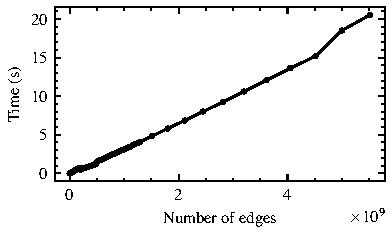
\includegraphics[width=\linewidth]{assets/timing.pdf}
    \caption{Performance of the GPU code for different number of nodes $n$. Number of edges via \eqref{eq:num-edges}.}
    \label{fig:timing}
\end{figure}

\vspace{-1.5em}

To test the performance of the GPU code, we measure the kernel execution time (including copying the results back to the host) for a range of number of nodes $n$ in the graph. For every $n$, we measure the duration 12 times\footnote{After every run, the device is re-initialized. Furthermore, we wait \qty{2}{\s} after every run before a new one starts.} and calculate mean and variance. The results are depicted in \autoref{fig:timing}. The variance is not shown as it is too small to be visible (always less than \qty{1}{\ms}). For $20,000$ words, the GPU code takes $\qty{484}{\ms}$ on average, while the CPU implementation needs $\qty{42}{\s}$. Up to $100,000$ nodes (\ie up to almost 5 billion edges), the GPU implementation takes less than \qty{20}{\s}. \autoref{fig:timing} also reveals the linear trend of time with increasing number of edges, which was to be expected since a thread is launched for every edge.

Our CUDA implementation is limited by the global memory (\qty{6}{\giga\byte} for the GPU at hand). This memory is used to store the resulting edge weights, \ie one byte per edge. The maximum number of edges we can handle is therefore the available memory divided by 1~byte. To obtain the corresponding number of nodes, we solve \eqref{eq:num-edges} for~$n$:
\begin{align}
    n = \frac{1}{2} + \sqrt{\frac{1}{4} + 2 \cdot \text{num edges}}
\end{align}
On the GPU at hand, we can handle up to around 107,000 nodes (mean time $\approx \qty{21.3}{\s}$) before experiencing \q{CUDA out of memory errors}. Currently we detect the limit, but do not implement a mechanism to go beyond it. One way could to be to detect the error, then copy the results back to the host and continue the computation while shifting the index back to $0$. The results are then concatenated on the host. For the further evaluation, we shall content ourselves with the results for the first 100,000 words, which already contain a lot of information of the French language. The binary file holding only the edge weights in row-major order, is \qty{4.66}{\giga\byte} in size.

\textbf{Graph application.} \autoref{fig:hist} shows the histogram of edge weights. It strongly resembles a normal distribution, which is probably due to how word lengths are distributed in the language. Note that the minimum and maximum achievable alignment score for a word pair depends on the word lengths. To efface this dependency, we normalize every score by dividing by $\max(\text{len}(A), \text{len}(B))$ and then multiply by 100. The resulting histogram is shown in \autoref{fig:hist-norm}. It does not resemble a normal distribution anymore. Most nodes have the smallest score of $-100$. There is a gap of around width 10 around edge weight 0 that we have no explanation for. The global trend is that many edges have a strong negative edge weight, while a smaller proportion have a strongly positive one.\label{paragraph:normalization}

The binary edge file is converted to a CSV file and imported into the open-source graph visualization software \href{https://gephi.org/}{Gephi}. As Gephi is far from being able to display 5 billion edges at the same time (let alone import such a file), we have to select specific ranges of edge weights we are interested in. We focus on the positive edge weights as they indicate a higher similarity between words.

Gephi implements various force-directed graph drawing algorithms that can help us gain a better understanding of the data. The principle of these algorithms is that nodes repulse each other, while edges act as springs to pull connected nodes together (taking into account the edge weights). Here, we exclusively use the algorithm by Yifan Hu\footnote{\href{http://yifanhu.net/PUB/graph_draw_small.pdf}{Efficient and High Quality Force-Directed Graph Drawing} by Yifan Hu in 2006.} as we found it to be the most efficient and reliable for our data. Furthermore, we run a modularity analysis using the Louvain method\footnote{\href{https://arxiv.org/abs/0803.0476}{Fast unfolding of communities in large networks} by Vincent Blondel et al.} implemented in Gephi. This method is used to detect communities in the graph, \ie groups of nodes that are more connected to each other than to the rest of the graph. We color the nodes according to the community they belong to (colors don't match between \textit{different} graphs in the following).

% \vfill\null

\begin{figure}[H]
    \centering
    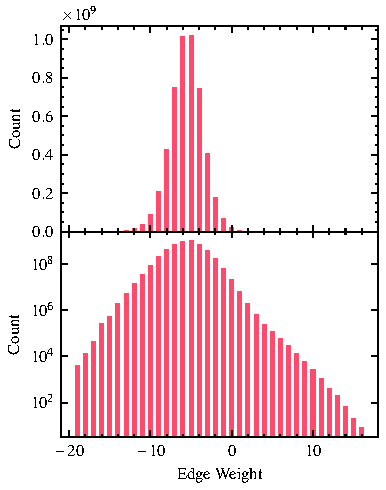
\includegraphics[width=\linewidth]{assets/edge_weights.pdf}
    \caption{Histogram of edge weights (linear and logarithmic scale). Mean: $-1.5$, range: $[-19, 16]$.}
    \label{fig:hist}
\end{figure}

% \vspace{-1em}

\begin{figure}[H]
    \centering
    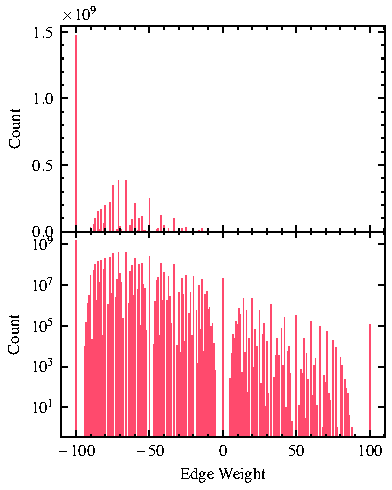
\includegraphics[width=\linewidth]{assets/edge_weights-normalized.pdf}
    \caption{Histogram of normalized edge weights. Linear and logarithmic scale.}
    \label{fig:hist-norm}
\end{figure}

\vfill\null
\columnbreak

\begin{figure*}[t]
    \centering
    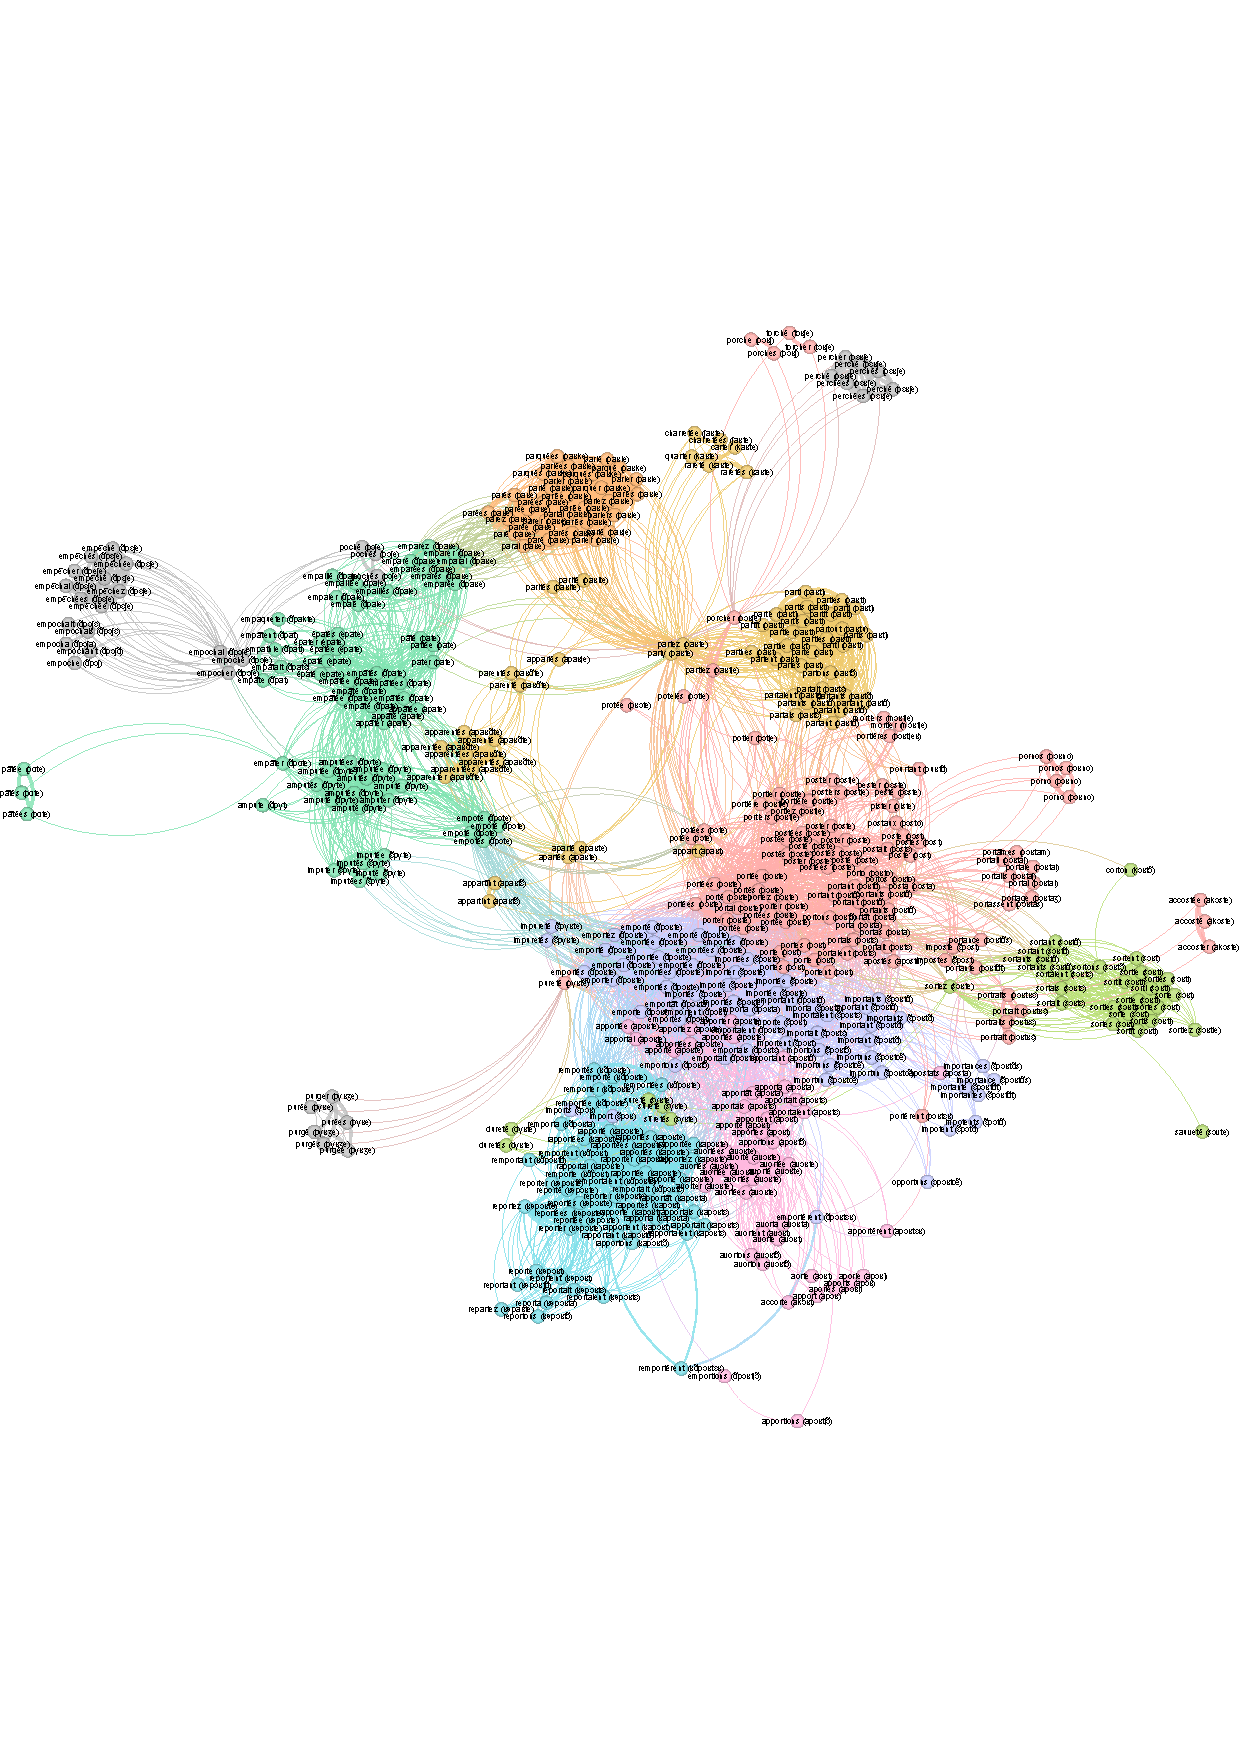
\includegraphics[width=\textwidth, trim=0cm 5.5cm 0cm 5.5cm, clip]{assets/emporter-ego.pdf}
    \caption{Ego-network (depth 3) of the word \textit{emporter} (to take away) for edge weights in the range $[60,100]$. This subgraph contains 449 nodes and 5921 edges.}
    \label{fig:emporter-ego}
\end{figure*}

\begin{figure}[H]
    \centering
    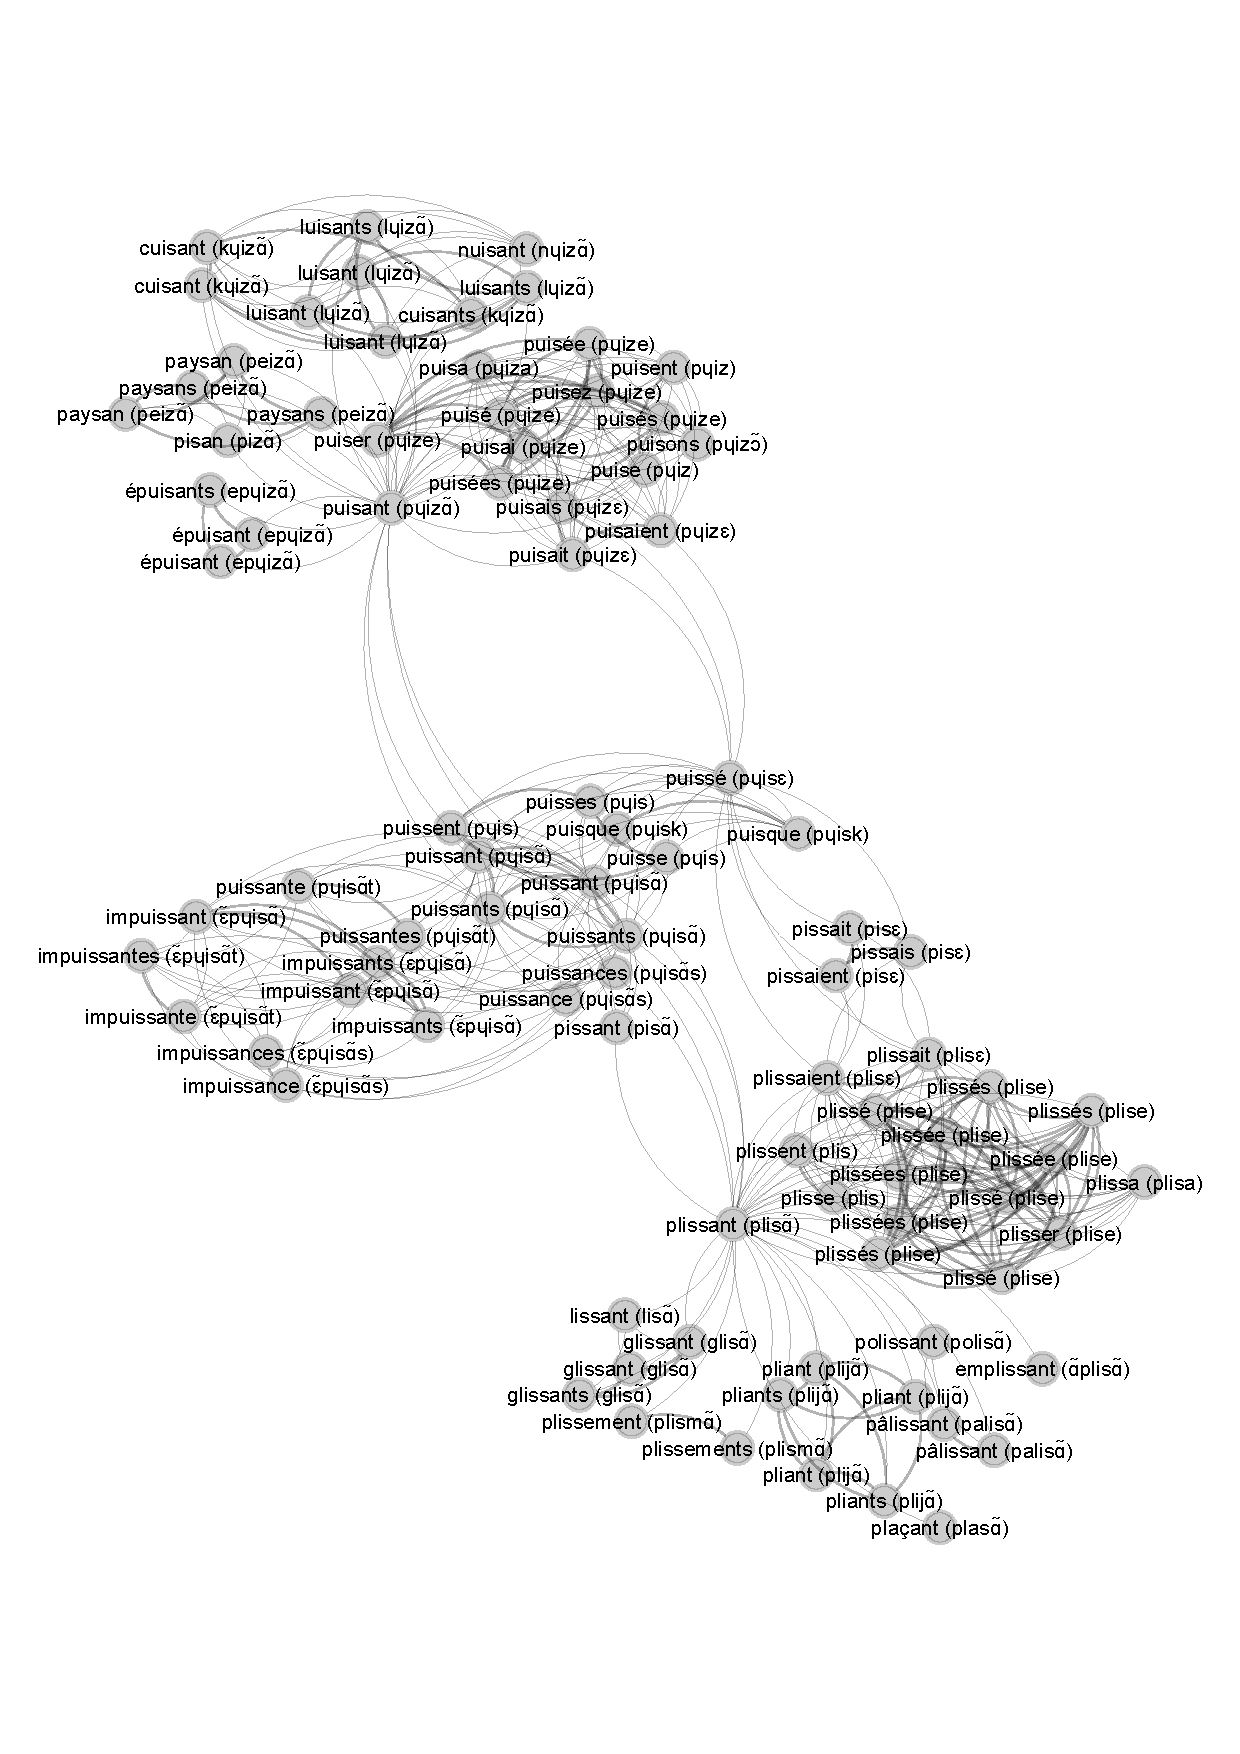
\includegraphics[width=\linewidth, trim=1cm 3.4cm 0.5cm 3.2cm, clip]{assets/puissant-ego.pdf}
    \caption{Ego-network (depth 3) of the word \textit{puissant}.}
    \label{fig:puissant-ego}
\end{figure}

\begin{figure}[H]
    \centering
    \includegraphics[width=\linewidth, trim=1cm 4.8cm 0.5cm 3.2cm, clip]{assets/étirer.pdf}
    \caption{Ego-network (depth 3) of the word \textit{étirer} for edge weights in the range $[40,49]$.}
    \label{fig:etirer-ego}
\end{figure}

Some resulting ego-networks are shown in figures \ref{fig:emporter-ego}, \ref{fig:puissant-ego} and \ref{fig:etirer-ego}. These graphs are constructed by locating neighbors of a word, then finding the neighbors of these neighbors up to a depth of~3. Different slices of edge weights are used, \eg in \autoref{fig:emporter-ego}, we have filtered the graph for edge weights in the range $[60,100]$ beforehand, which account for a total of 458,529 edges. The networks clearly show that our implementation is working correctly and that Needleman-Wunsch indeed gives a meaningful metric in this context.

\begin{itemize}[leftmargin=0cm]
    \item Words with the same pronunciation are as close as possible to each other and reside in the same community. In \autoref{fig:etirer-ego}, the words \textit{étudier}, \textit{étudient}, \textit{étudié}, \textit{étudiai}, \textit{étudiées} etc. are close to each other. In \autoref{fig:emporter-ego}, inside the red group in the middle-right part, we find different adjective endings for the word \textit{porté} (corresponding to gender and number of the noun it describes, \ie adjective agreement): porté, portée, portés, portées. We also find the words \textit{porter} and \textit{portez} here with the same prononciation as \textit{porté}. Note that it is claimed that \textit{portai} has the exact same prononciation, which is not correct (the last phoneme is different). This also shows that the dataset itself is not perfect and may contain errors. 
    
    \item Of greater interest are similar sounding words; as hoped for, they are close to each other in the graph. For example, in \autoref{fig:emporter-ego}, we find edges like \textit{emporté} -- \textit{porter}, \textit{emporté} -- \textit{importé}, \textit{importé} -- \textit{impureté} and \textit{impureté -- pureté}. It is also remarkable that words in one group almost exclusively start with the same letter and correspond to the same word root: \textit{sortir} in the green group on the right, \textit{porter} and \textit{poster} in the red group, \textit{emporter} and \textit{importer} in the violet group, \textit{apporter} in the purple group, \textit{rapporter}, \textit{reporter} and \textit{remporter} in the blue group etc.
    
    \item There are stronger and weaker connections between words. In \autoref{fig:puissant-ego}, the edge between \textit{puisant}\footnote{Note that this is not missing an additional \textit{s}. This is the word in a phrase like \q{en \textit{puisant} de l'eau, ...}.} -- \textit{épuisant} has weight $\nicefrac{200}{3}\approx 66.7$ (after normalization), while that of \textit{puisant} -- \textit{paysans} has the smaller weight $\nicefrac{300}{5} = 60$.
    \begin{table}[H]
        \centering
        \begin{tabular}{l*{6}{>{\centering\arraybackslash}p{0.2cm}}}
            \toprule
            \textit{paysans}
            & & \textipa{p} & \textipa{e} & \textipa{i} & \textipa{z} & \textipa{A}\\
            \midrule
            \textit{puisant}
            & & \textipa{p} & \textipa{\textturnh} & \textipa{i} & \textipa{z} & \textipa{\~A}\\
            \midrule
            \textit{épuisant}
            & \textipa{e} & \textipa{p} & \textipa{\textturnh} & \textipa{i} & \textipa{z} & \textipa{\~A}\\
            \bottomrule
        \end{tabular}
        \caption{Optimal alignment of three words.}
        \label{tab:align-puisant}
    \end{table}
    \vspace{-1.3em}

    \autoref{tab:align-puisant} shows the corresponding optimal alignments. With a match score of $1$, a mismatch score of $-1$ and a gap penalty $p=-1$, we find a score of~3 (\textit{puisant} -- \textit{paysans}) and 4 (\textit{puisant} -- \textit{épuisant}). With the normalization discussed on \autopageref{paragraph:normalization}, we indeed obtain the aforementioned edge weights. This example also illustrates that fine-tuning match/mismatch score and gap penalty is important to obtain meaningful results. One might want a greater distance between \textit{paysans} and \textit{puisant} since the \textipa{/u/} is replaced by the very different sounding \textipa{/a/}. Furthermore, the match/mismatch scores can be adjusted for every pair of phonemes to reflect the subtleties of a language. This can be done by changing the coefficients in the similarity matrix (see \autoref{algstep:sim} of \autoref{alg:needleman-wunsch}). In this document, we limit ourselves to the default scoring matrix ($1$ on the diagonals, $-1$ elsewhere).
\end{itemize}

Furthermore, we want to broaden the view by considering a bigger graph, see \autoref{fig:big-view} containing 306,473 edges with normalized weights 8, 9 or 10.


\vfill\null

\begin{figure}[H]
    \centering
    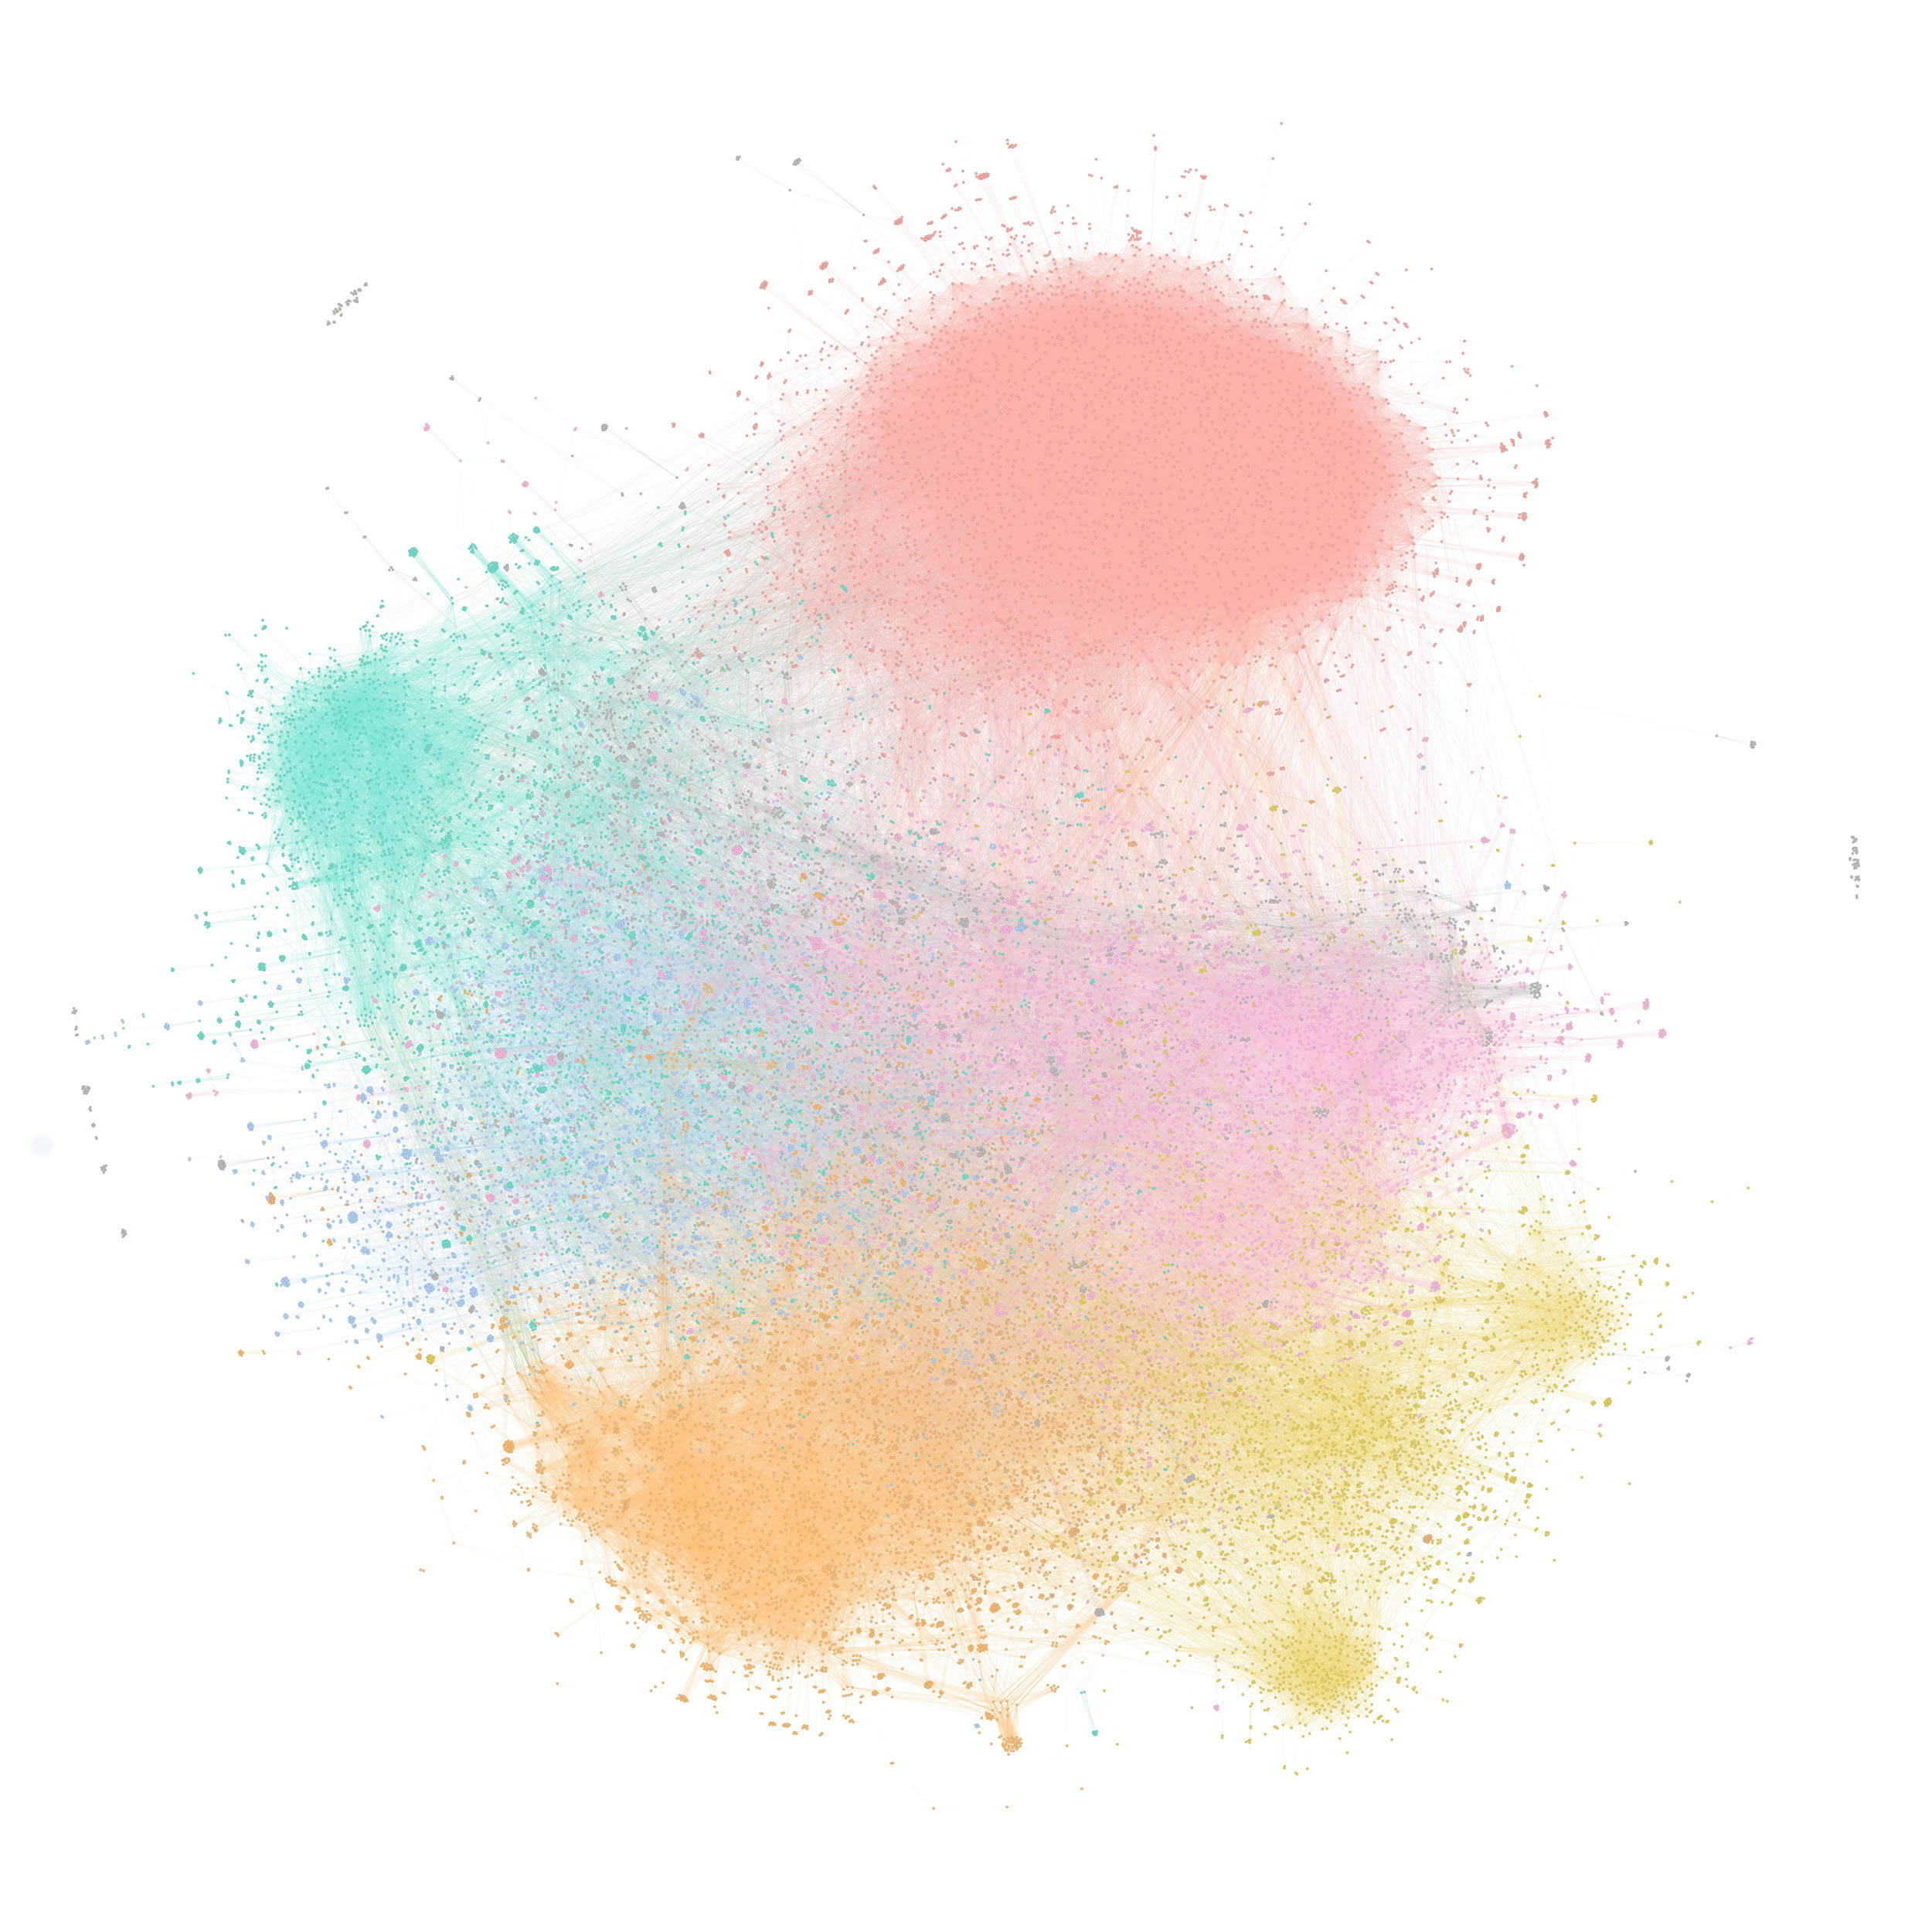
\includegraphics[width=\linewidth, trim=1cm 4.8cm 0.5cm 3.2cm, clip]{assets/big view-min-min.jpg}
    \caption{Overview of the graph containing edge weights in the range $[8,10]$. 30,185 nodes and 306,473 edges are shown.}
    \label{fig:big-view}
\end{figure}






% ForceAtlas2 algorithm. The neighbors of the word \q{glace} and \q{prévoir} are shown in \autoref{fig:neighbors}. For bigger graphs than that, Gephi is not able to handle the amount of data anymore.

Having translated the problem into a graph structure also allows us to use graph algorithms to discover interesting properties. As an example, Gephi implements the \textit{shortest path algorithm}: users can click on two words and the shortest path between them is calculated and shown in the graph. Beforehand, we filtered the graph to only include the most strong edges. With this, we can find chains like the following (read them aloud to hear the phonetic similarity):
\begin{itemize}
    \item trottoir $\rightarrow$ entrevoir $\rightarrow$ devoir $\rightarrow$ voire $\rightarrow$ voile $\rightarrow$ val $\rightarrow$ valait $\rightarrow$ fallait $\rightarrow$ falaise
    \item falaise $\rightarrow$ fallait $\rightarrow$ palais $\rightarrow$ passais $\rightarrow$ dépassait $\rightarrow$ dépendait $\rightarrow$ répondait $\rightarrow$ répond $\rightarrow$ raison $\rightarrow$ maison
    \item confusion $\rightarrow$ conclusion $\rightarrow$ exclusion $\rightarrow$ explosion $\rightarrow$ exposition $\rightarrow$ explications $\rightarrow$ respiration $\rightarrow$ précipitation $\rightarrow$ présentation $\rightarrow$ présenta $\rightarrow$ présente $\rightarrow$ présence $\rightarrow$ présidence $\rightarrow$ résidence $\rightarrow$ résistance $\rightarrow$ existence
\end{itemize}

% \section{Conclusion}
\label{sec:conclusion}

% Computation
% - stencil computation -> try to parallelize at finer granularity
% - Calculate more words at the same time by filtering uninteresting weights
%   directly (for this purpose generate histogram of weights distribution)

% Domain Level
% - fine-tune similarity matrix for language subtleties
% - experiment with parameters: match/mismatch score, gap penalty p
% - consider lexeme as those are more interesting
% - multiple languages (!)
% - offer online service to show neighbors of a word in a ego network
%   (users can search for a word)

% - more graph theory applications other than shortest path?


% normalize score to word length n+m
\end{multicols*}

\printglossary[type=\acronymtype]

\end{document}
